%%This is a very basic article template.
%%There is just one section and two subsections.
%\documentclass[12pt,oneside,a4paper,doublespacing]{article} % for submission
\documentclass[12pt,oneside,a4paper]{article} % for sharing
\usepackage{apacite}
\usepackage{appendix}
\usepackage{amsmath}
\usepackage{amsthm}
 
\usepackage{amssymb} % for approx greater than
\usepackage{caption}
\usepackage{placeins}
\usepackage{graphicx}
% graphicx loaded by adjustbox?
%\usepackage[export]{adjustbox} % for bottom alignment in m{} columns, package
% not \usepackage{graphbox} % for bottom alignment in m{} columns, package not
% found\ldots
\usepackage{subcaption}
%\usepackage{subfig}
\usepackage{longtable}
\usepackage{setspace}
%\usepackage{tikz}
\usepackage{booktabs}
\usepackage{tabularx}
\usepackage{xcolor,colortbl}
\usepackage{chngpage}
%\usepackage[active,tightpage]{preview}
\usepackage{natbib}
\bibpunct{(}{)}{,}{a}{}{;} 
\usepackage{url}
\usepackage{nth}
\usepackage{authblk}
%\usepackage[export]{adjustbox}
\usepackage[most]{tcolorbox}
%\usepackage{hyperref}
%\usepackage{color}
%\usepackage{fontspec}
%\usepackage{pdfsync}
\usepackage[normalem]{ulem}
\usepackage{amsfonts}
%\renewcommand{\listtablename}{List of Appendix Tables}
\newcolumntype{C}[1]{>{\centering\let\newline\\\arraybackslash\hspace{0pt}}m{#1}}
\newcolumntype{L}[1]{>{\raggedright\let\newline\\\arraybackslash\hspace{0pt}}m{#1}}
% working on this need to concatenate file name based on sex and variable name
%\newcommand\Cell[1]{{\raisebox{-0.05in}{\includegraphics[height=.2in,width=.2in]{Figures/ColorCodes/\expandafter#1}}}}  

% otherwise it ignores this big table!
%\DeclareDelayedFloatFlavour*{longtable}{table}
\usepackage[margin=1in]{geometry}
%\doublespacing % for review

% line numbers to make review easier
%\usepackage{lineno}
%\linenumbers

\usepackage{soul}% for \st{}

% for appendix definition environment
\theoremstyle{definition}
\newtheorem{definition}{Definition}[section]
\newtheorem{theorem}{Theorem}[section]
\newtheorem{corollary}{Corollary}[theorem]
%\newtheorem{proof}{Proof}[theorem]
%%%%%%%%%%%%%%%%%%%%%%%%%%%%%%%%%%%%%%%%%%%%%%%%%%%%%%%%%%%%%%%%%%%%%%%%%%%%%
% setting color to letters affects spacing. Here's a hack I found here:
% http://tex.stackexchange.com/questions/212736/change-letter-colour-without-losing-letter-spacing
%\DeclareRobustCommand{\spacedallcaps}[1]{\MakeUppercase{\textsc{#1}}} % all
% caps with better spacing

\colorlet{rd}{red}
\colorlet{bl}{blue}

%%%%%%%%%%%%%%%%%%%%%%%%%%%%%%%%%%%%%%%%%%%%%%%%%%%%%%%%%%%%%%%%%%%%%%%%%%%%%%

\newcommand\ackn[1]{%
  \begingroup
  \renewcommand\thefootnote{}\footnote{#1}%
  \addtocounter{footnote}{-1}%
  \endgroup
}
\newcommand\vt[1]{\textcolor{rd}{#1}}
\newcommand\eg[1]{\textcolor{bl}{#1}}

\newcommand\tg[1]{\includegraphics[scale=.5]{Figures/triadtable/triad#1.pdf}}
\newcommand\tgh[1]{\raisebox{-.25\height}{\includegraphics[scale=.3]{Figures/triadtable/triad#1.pdf}}}


\newcommand{\Ed}[1]{\includegraphics[scale=.45]{{Figures/TimeLinesAndGraphs/edgep#1}.pdf}}
\newcommand{\Tl}[1]{\includegraphics[scale=.45]{{Figures/TimeLinesAndGraphs/linep#1}.pdf}}
\newcommand{\St}[1]{\includegraphics[scale=.45]{{Figures/TimeLinesAndGraphs/starp#1}.pdf}}


\defcitealias{HMD}{HMD 2016}

% junk for longtable caption
\AtBeginEnvironment{longtable}{\linespread{1}\selectfont}
\setlength{\LTcapwidth}{\linewidth}

% sort van Raalte properly
% #1: sorting key, #2: prefix for citation, #3: prefix for bibliography
\DeclareRobustCommand{\VAN}[3]{#2} % set up for citation

%%%%%%%%%%%%%%%%%%%%%%%%%%%%%%%
\begin{document}

\title{A unified framework of demographic time}
%\author{author(s) redacted}
\author[1]{Tim Riffe\thanks{riffe@demogr.mpg.de}}
\author[2,3]{Jonas Sch{\"o}ley}
\author[2,3]{Francisco Villavicencio}
\affil[1]{Max Planck Institute for Demographic Research}
\affil[2]{University of Southern Denmark}
\affil[3]{Max-Planck Odense Center on the Biodemography of Aging}

%\author{[Authors]}

\maketitle
\pagebreak
\begin{abstract}
Demographic thought and practice is largely conditioned by the Lexis diagram,
a two-dimensional graphical representation of the identity between age,
period, and birth cohort. This relationship does not account for remaining years
of life, total length of life, or time of death, whose use in
demographic research is both underrepresented and incompletely situated. We
describe an identity between these six demographic time measures, and generalize
this relationship to time measures derived from an arbitrary number of events in
calendar time. We describe the sub-identities that pertain to the six-way
demographic time identity, and provide a topological overview of the diagrams that pertain to
these identities in both two and three dimensions. We provide an application of
this framework on the measurement of late-life disability prevalence. 


\smallskip
\noindent \textbf{Keywords.} Age structure, formal demography, data
visualization, age period cohort.%\ackn{The work reported in this manuscript
%began while the first author was at the Department of Demography at the
% University of California, Berkeley, and was supported by the U.S.
%National Institute On Aging of the National Institutes of Health under award
%numbers R01-AG011552 and R01-AG040245. The content is solely the responsibility
% of the authors and does not necessarily represent the official views of the
% funding agencies. We also wish to thank two anonymous reviews for comments
% that greatly improved the paper.}
\end{abstract}

%\pagebreak

\section{Introduction}
In the course of training, all demographers are introduced
to the Lexis diagram, a convenient graphical identity between the three main
time measures used to structure demographic stocks and flows: Age, period, and
birth cohort. This representation does not account for time of death, time until
death, or length of life, which may be of interest to researchers \st{and
policy makers} as structuring rather than random variables in order to capture
variation in demographic data.
\st{This popular representation does not account for remaining years of life and other related time indices that may be of interest to researchers and
policy makers.} 

We wish to draw attention to three time indices that are complementary to age
(A), period (P) and birth cohort (C). The first such index is time-to-death,
which we refer to as ``thanatological age'' (T) in contrast to ``chronological
age'' (A). The second index is death cohort (D), which groups all individuals
(of different ages) dying in the same time period. Finally, lifespan (L) or
individual age-at-death itself is an index by which data may be structured.
We therefore have six time measures in total to relate. We call these measures of demographic
time because each, except period, depends on the timing of birth, death, or
both.

The Lexis diagram can be understood as an APC plane
that relates age, period, and birth cohort. Other such planes are
also identifiable.
The ``thanatological'' ``dual'' of APC is an identity between thanatological
age, period, and death cohort, TPD. A third identity relates thanatological age,
chronological age, and lifespan, TAL. A fourth identity relates lifespan, birth
cohort, and death cohort, LCD. We call three-way identities of this sort ``triad identities''.

Each of these four triad identities (APC, TPD, TAL, and LCD) is sufficiently
described by any two of its constituent indices\st{, making the third index
redundant}. For instance, if the exact age of an individual at a particular
time is known, the birth cohort to which he or she belongs can be immediately derived. Each of these four identities also lacks a major dimension of time. The TAL identity lacks calendar time, the LCD identity is ageless, APC lacks an endpoint in time, and TPD lacks a starting point in time.
To our knowledge, the only triad identity that has received serious
treatment at the time of this writing is the APC identity. Different
aspects of the APC identity have been discussed since at least 1868
\citep{knapp1868ermittlung}, and discussion remains lively today. Here we relate the six major indices of time in a geometric identity, in much the same spirit as the work on APC relationships done between the late
1860s and mid 1880s.\footnote{See e.g., \citet{keiding2011age} for an overview of that literature.} 

Our goal is to describe the geometric identity between all
six measures of demographic time, a hexad identity, that may be useful or an intuitive
referent for demographers in the same way as the Lexis diagram. At the same
time, this identity relates the four triad identities we have mentioned. We give a bottom-up
description of how such temporal identities can be derived from an
arbitrary number of events in calendar time in a simple and general
event-duration relationship. These more general event-duration foundations
facilitate comparison of the demographic time framework with other temporal designs found in the
literature, such as the higher-order temporal model of \citet{brinks2014lexis},
or the marriage cohort hexad identity described by \citet{lexis1875einleitung}.
The framework we describe is general and adaptable for such event history scenarios.
We begin by defining some terms used throughout the manuscript.
We then explore all combinations of two time measures, the dyadic relationships, followed by the four triad identities, and
finally the hexad identity. We give a systematic topological overview of the
different elements of demographic time. 

Just as the Lexis diagram has been a fundamental instrument to
teach demography for decades, we hope that the demographic time measures and
their graphical depictions presented here will be helpful to teachers and
young demographers. The temporal relationships we describe will also be useful
for researchers to better detect and understand patterns data, and for
methodologists to better account for the structure of data in demographic
methods or statistical designs.

\section{Definitions}
\subsection{Technical terminology}
In describing this relationship we attempt to adhere to a rigorous
terminology.
The following list describes some of the more important terms we use.
\begin{description}
\item[Demographic time measures] are any of the six time indices discussed to
describe demographic time: chronological age (A), period (P), birth cohort (C), thanatological age (T), lifespan (L), and death cohort (D).
\item[Dyads, triads, and hexads] are any set of two, three, or six unique time
measures, respectively.
\item[A triad identity] is a triad with the property that each of its members
can be derived from the other two with no additional information. There are four triad
identities: APC, TPD, TAL, and LCD.
%\item[A hexad identity] is a unique combination of the six time measures.
\item[A temporal plane] is any $(x,y)$-mapping of a dyad of time measures.
\end{description}
Using this terminology, we say that the ``Lexis'' measures
constitute a triad identity between chronological age, period, and birth cohort. Each dyad
combination of elements in this identity can be mapped to a
temporal plane, the Lexis diagram. If we know that Mindel turned 50 on the
\nth{21} of May, 1963, then we also can derive that she was born on the \nth{21} of
May, 1913. Hence, any two pieces of information in this case will give the
third, and the same holds for the other triad identities.

\FloatBarrier
\subsection{Time measures}
\FloatBarrier
We describe time in terms of years, the dominant time scale for human
demography, although all relationships are scalable to any time unit. We therefore speak of calendar time. We also describe the framework in terms
of human lifespans, although it applies in a more general sense to any durations
observed over time. This is to say, birth may be translated to entry, and death
to exit, or any other absorbing state. The six measures of time we consider are
defined in Table~\ref{tab:sixdefs}, both in the demographic sense we describe, as well as in a more general event history interpretation.

\FloatBarrier
\begin{table}[ht!]
\centering
\caption{Definitions of the six time measures.}
\label{tab:sixdefs}
\begin{adjustwidth}{0em}{0em}
\begin{tabular}{lcll}
\hline 
\textbf{Time measure} & \textbf{Short} & \textbf{Demographic def.} &
\textbf{Event history def.}\\
\hline 
chronological age & A & Time since birth & Time since start of exposure \\
period & P & calendar time & calendar time \\
birth cohort & C & calendar time of birth & calendar time of exposure start \\
thanatological age & T & time until death & time until event \\
death cohort & D & calendar time of death & calendar time of event \\
lifespan & L & duration of life & duration of exposure \\
\end{tabular}
\end{adjustwidth}
\end{table}

The concepts of thanatological age and death cohorts are likely less familiar to
readers than the other measures we consider. Thanatological age invokes the
remaining lifetime until death, the information approximated with life
expectancy. This term is sometimes referred to in the literature as life left,
time to death, remaining lifespan, follow-up duration, residual life, or
reverse time.
Chronological and thanatological age are in this way complementary, duals. On the other hand, cohorts in general associate individuals that share a characteristic. In demography the grouping characteristic is often a combination of place and time, such as a cohort of young demographers passing through a particular graduate program. These concepts are analogous to the ideas of birth and death cohorts we use here. The deaths of a given year are not usually referred to as a death cohort, although this concept was already introduced by \cite{brouard1986} as ``g\'en\'eration de d\'ec\`es'' in a retrospective study of the French population during the twentieth century. In the time preceding death, the members of a given death cohort have much in common, despite heterogeneity with respect to time of birth. If the reader accepts this premise, then the abstract construct of a death cohort is also meaningful in the way that other cohort measures are. In event history or non-human contexts, anologs to death cohorts in this framework may be even more meaningful.

Much of the work of demography is directed at the study of lifespan. Lifespan is
synonymous both with longevity, chronological age at death, and thanatological
age at birth. One's ultimate completed lifespan is constant throughout life,
though we have no knowledge of it until death: It is assigned retrospectively.
Demographers have more often used lifespan or age-at-death as a measure of
mortality, or similar, than as a measure on which to compare individuals or
structure data.

Treating lifespan,
death cohorts, and thanatological age as temporal structuring variables
enables new classes of comparisons, models of understanding, and discovery,
akin to those unlocked by breaking down demographic phenomena by chronological age,
period, and birth cohort. The following sections, in this sense, provide an
exhaustive classification of the ways in which these six measures of time can be juxtaposed to such ends.

%FloatBarrier

\section{From dyads to the triad identities}
\label{sec:dyads2diagrams}
We distinguish between two kinds of dyads: informative dyads and uninformative dyads. Informative dyads are any pair of measures from which a third time measure
can be derived, forming a triad identity. There are
$15=\binom{6}{2}$ possible dyads in our set of time measures, 12 of which are
informative, and three of which have no derived time measure, and are therefore
called uninformative. For instance, if we take the dyad TA, L is the derived
measure, and TAL the corresponding triad identity. In
contrast, nothing can be derived from the LP dyad: You can have an eventual lifespan of 100 in the year 2016 and still be alive with the same eventual lifespan in 2017.

In this section we systematically map each dyad to its temporal plane, and we
synthesize these into the four primary identities and their essential diagrams.
We first discuss the choice between mapping dyads to Cartesian coordinates or to
isotropic coordinates, which constrain the scales of all measures to be equal.
We then systematically render the 15 dyad-based diagrams that can be derived from the six time measures. Of these 15, 12 diagrams can be distilled into just four, the triad identity diagrams. Each
triad identity diagram is then briefly discussed with suggested or speculated
applications.

\subsection{The question of mapping}
Any mapping of two time measures to an ($x,y$) coordinate
system constitutes a temporal plane. If the two given time measures are members of the same triad identity, the third member is a derived
measure. If we assign A to $y$ and P to $x$, thereby implying C (and the APC
triad identity) we state this relationship explicitly by writing
AP(C).
The temporal plane that corresponds to this informative dyad is the contemporary representation of the
Lexis diagram \citep{lexis1875einleitung, pressat1961analyse}. The informative
dyads AC(P) and CP(A) also belong to the Lexis identity, but imply different
less-common rotations and projections of the Lexis diagram.\footnote{While
uncommon as diagram orientations, these latter two dyads are used to tabulate
data for different kinds of rates and probabilities. Measures
based on the AC dydad are variously referred to as Type III rates
\citep{caselli2005demography} or vertical parallelograms \citep{HMDMP}. The CP
dyad delineates Type II rates \citep{caselli2005demography}, also known as
horizontal parallelograms, for instance used to calculate cohort lifetables in the Human
Mortality Database \citep{HMDMP}. }

For each dyad there is a fundamental question of how to map the constituent
coordinates to a Cartesian temporal plane. Typically one forces parity between time units within
a specified dyad, mapping one element directly to $x$ and the second element
directly to $y$, resulting in a 90$^\circ$ angle between the $x$ and $y$
axes. In this case it is conventional to force a unity aspect ratio
between the $x$ and $y$ axes, such that the derived measure, if any, is then
\textit{accidentally} present in a 45$^\circ$ ascending or descending angle,
depending on the dyad and axis orientation. 

It has long been noted \citep{lexis1875einleitung, perozzo1880della} that the
derived time measure (usually birth cohort) is longer than either the age or period axes when plotted at 45$^\circ$.
If a right angle and unity aspect ratio is forced between the dyad, the derived measure is always stretched by
$\sqrt{2}$, or 41\%. In the case of informative dyads, another
logical mapping is to translate to $(x,y)$ coordinates that force 60$^\circ$
angles between the three measures. Such a mapping ensures that the spatial units are equal for the three measures, and we therefore refer to it as the isotropic mapping. The isotropic mapping
is comparable to using ternary or barycentric coordinate systems. 
The primary justification for isotropic demographic surfaces comes from
a data visualization perspective, where it may be hypothesized that the
 viewer's ability to compare slopes is hindered if time coordinates are not on
 the same scale. Under the isotropic representation, the three variants of each
 triad identity are simple rotations of one another, and they require no
 rescaling. In this paper, all two-dimensional diagrams are rendered in
 Cartesian rather than isotropic coordinates.

\subsection{Dyads to diagrams}
Each of the 15 dyads, an explanation or simple example,
and the corresponding diagram representations are summarized in
Table~\ref{tab:dyads}. Each informative dyad is a subset consisting of two
elements from one of the four triad identities (APC, TPD, TAL, LCD), which we
analyze in detail in further sections. The uninformative dyads are simply pairs
of time measures that do not have a derived measure, and therefore are not
contained in any of these four triad identities.
\pagebreak

\begin{longtable}{m{0.15\textwidth}L{0.4\textwidth}m{0.2\textwidth}}%m{0.2\textwidth}}
  \caption{All dyadic juxtapositions of the six measures of demographic time.}
  \label{tab:dyads}\\
 
  \toprule
  \multicolumn{3}{m{0.9\textwidth}}{\footnotesize \emph{Note:} The temporal
  planes are named after the two given time scales. The derived scale is appended in parentheses. Contrary to mathematical convention we name the ordinate scale first and the abscissa scale second. This is to be consistent with the established $APC$ and $ACP$ terms.} \\
  \midrule
  \multicolumn{1}{c}{Relationship} & \multicolumn{1}{c}{Description} &
  \multicolumn{1}{c}{Cartesian} \\%& \multicolumn{1}{c}{Isotropic} \\
  \midrule
  %%%%%%%%%%%%%%%%%%%%%%%%%%%%%%%%%%%%%%%%%%%%%%%%%%%%%%%%%%%%%%%%%%%%%%%%%%%%%
  \multicolumn{3}{c}{\textsc{Variants of APC}} \\
  \midrule
  %%%% APc
  $$\begin{aligned}
    &AP(C) \\
    &C = P - A
  \end{aligned}$$ &
  The AP(C) temporal plane constitutes the classical Lexis diagram. &
  \includegraphics[scale=.5]{Figures/DiagramTable/AP_rt.pdf}
  %&
  %\includegraphics[scale=.5]{Figures/DiagramTable/AP_iso.pdf}
  \\
  %%%% ACp
  $$\begin{aligned}
    &AC(P) \\
    &P = C + A
  \end{aligned}$$ &
  The AC(P) temporal plane is equivalent to the Lexis diagram except birth
  cohort is given and period is derived rather than the other way around. &
  \includegraphics[scale=.5]{Figures/DiagramTable/AC_rt.pdf} %& 
  %\includegraphics[scale=.5]{Figures/DiagramTable/AC_iso.pdf} 
   \\
  %%%% CPa
  $$\begin{aligned}
    &CP(A) \\
    &A = P - C
  \end{aligned}$$ &
  The CP(A) temporal plane is equivalent to the Lexis diagram except birth
  cohorts are given and age is derived rather than the other way around. &
  \includegraphics[scale=.5]{Figures/DiagramTable/CP_rt.pdf} %& 
  %\includegraphics[scale=.5]{Figures/DiagramTable/CP_iso.pdf}  
  \\
  \midrule
  %%%%%%%%%%%%%%%%%%%%%%%%%%%%%%%%%%%%%%%%%%%%%%%%%%%%%%%%%%%%%%%%%%%%%%%%%%%%%
  \multicolumn{3}{c}{\textsc{Variants of TPD}} \\
  \midrule
  %%%% TPd
  $$\begin{aligned}
    &TP(D) \\
    &D = P + T
  \end{aligned}$$ &
  Helen had 30 years of life left (T) in 1971 (P) and therefore belonged to the 2001 death cohort (D) &
  \includegraphics[scale=.5]{Figures/DiagramTable/TP_rt.pdf} %&
  %\includegraphics[scale=.5]{Figures/DiagramTable/TP_iso.pdf} 
   \\
  %%%% PDt
  $$\begin{aligned}
    &PD(T) \\
    &T = D - P
  \end{aligned}$$ &
  Mindel died in 1973 (D). In 1953 (P) she had 20 years left to live (T). &
  \includegraphics[scale=.5]{Figures/DiagramTable/PD_rt.pdf} %&
  %\includegraphics[scale=.5]{Figures/DiagramTable/PD_iso.pdf} 
   \\
  %%%% TDp
  $$\begin{aligned}
    &TD(P) \\
    &P = D - T
  \end{aligned}$$ &
  Irene died in 1974 (D). When she had 30 remaining years of life (T) the year must have been 1944 (P). &
  \includegraphics[scale=.5]{Figures/DiagramTable/TD_rt.pdf} %&
  %\includegraphics[scale=.5]{Figures/DiagramTable/TD_iso.pdf}  
  \\
  \midrule
  %%%%%%%%%%%%%%%%%%%%%%%%%%%%%%%%%%%%%%%%%%%%%%%%%%%%%%%%%%%%%%%%%%%%%%%%%%%%%
  \multicolumn{3}{c}{\textsc{Variants of TAL}} \\
  \midrule
  %%%% TAl
  $$\begin{aligned}
    &TA(L) \\
    &L = T + A
  \end{aligned}$$ &
  The time already lived and the time still left sum up to the total lifespan. &
  \includegraphics[scale=.5]{Figures/DiagramTable/TA_rt.pdf} %&
  %\includegraphics[scale=.5]{Figures/DiagramTable/TA_iso.pdf}  
  \\
  %%%% TLa
  $$\begin{aligned}
    &TL(A) \\
    &A = L - T
  \end{aligned}$$ &
  Helen lived to the age of 86 (L). When she had 20 years left (T) she must have been 66 (A). &
  \includegraphics[scale=.5]{Figures/DiagramTable/TL_rt.pdf} %&
 % \includegraphics[scale=.5]{Figures/DiagramTable/TL_iso.pdf}  
 \\
  %%%% ALt
  $$\begin{aligned}
    &AL(T) \\
    &T = A - L
  \end{aligned}$$ &
  Tim is 34 years old (A) and will live to the age of 96 (L), leaving him 62 years (T) to settle affairs. &
  \includegraphics[scale=.5]{Figures/DiagramTable/AL_rt.pdf} %&
  %\includegraphics[scale=.5]{Figures/DiagramTable/AL_iso.pdf} \\
  \\
  \midrule
  %%%%%%%%%%%%%%%%%%%%%%%%%%%%%%%%%%%%%%%%%%%%%%%%%%%%%%%%%%%%%%%%%%%%%%%%%%%%%
  \multicolumn{3}{c}{\textsc{Variants of LCD}} \\
  \midrule
  %%%% LCd
  $$\begin{aligned}
    &LC(D) \\
    &D = C + L
  \end{aligned}$$ &
  \`{A}ngels was born in 1940 (C) and she lived to be 64 (L), implying an
  untimely death in 2004 (D) &
  \includegraphics[scale=.5]{Figures/DiagramTable/LC_rt.pdf} %&
  %\includegraphics[scale=.5]{Figures/DiagramTable/LC_iso.pdf}  
  \\
  %%%% CDl
  $$\begin{aligned}
    &CD(L) \\
    &L = D - C
  \end{aligned}$$ &
  Pascal was born in 1893 (C) and died in 1964 (D), implying a lifespan of 71 (L), or so. &
  \includegraphics[scale=.5]{Figures/DiagramTable/CD_rt.pdf} %&
  %\includegraphics[scale=.5]{Figures/DiagramTable/CD_iso.pdf}  
  \\
  %%%% LDc
  $$\begin{aligned}
    &LD(C) \\
    &C = D - L
  \end{aligned}$$ &
  Margaret died in Dec., 1995 (D) with a completed lifespan of 96 (L), putting her birth year in 1900 (C). &
  \includegraphics[scale=.5]{Figures/DiagramTable/LD_rt.pdf} %&
  %\includegraphics[scale=.5]{Figures/DiagramTable/LD_iso.pdf}  
  \\
  \midrule
  %%%%%%%%%%%%%%%%%%%%%%%%%%%%%%%%%%%%%%%%%%%%%%%%%%%%%%%%%%%%%%%%%%%%%%%%%%%%%
  \multicolumn{3}{c}{\textsc{The Uninformative Dyads}} \\
  \midrule
  %%%% LP
  LP(-) &
  The LP plane is \emph{non-informative}. No additional measures can be derived knowing just lifespan and period. &
  \includegraphics[scale=.5]{Figures/DiagramTable/LP_rt.pdf} %&
  %\includegraphics[scale=.5]{Figures/DiagramTable/LP_rt.pdf} 
  \\
  %%%% CT
  CT(-) &
  The CT plane is \emph{non-informative}. No additional measures can be derived
  knowing just birth cohort and thanatological age. &
  \includegraphics[scale=.5]{Figures/DiagramTable/CT_rt.pdf} \\
  %%%% AD
  AD(-) &
  The AD plane is \emph{non-informative}. No additional measures can be derived
  knowing just death cohort and age. &
  \includegraphics[scale=.5]{Figures/DiagramTable/AD_rt.pdf} 
\\
  \bottomrule
\end{longtable}

Most of what we know about how rates change over age and time comes
from the very first juxtaposition in Table~\ref{tab:dyads}, AP(C). While
CP(A) and AC(P) are statistically redundant when exact times are used, they
are not fully redundant if based on discrete double-classification of data, as
often provided in aggregated official statistics. Double classified data are
found on the APC diagram in the shape of squares (AP), horizontal parallelograms
(AC) and vertical paralellograms (PC), and
these are commonly used to compute different kinds of demographic
rates and probabilities \citep[][p. 63]{caselli2005demography}. The other dyadic
juxtapositions (involving the measures T, D, or L) can be considered as either
rare or novel ways of structuring or viewing temporal variation in demography,
and these imply new families of rates and probabilities.

\subsection{The triad identities}
\label{sec:triads}
There are $20=\binom{6}{3}$ ways to choose three time indices out of
six, of which four form a triad identity: APC, TPD, TAL, and LCD.
Given the three time measures from any of the
triad identities, one can derive no further time measures. If one selects three
random time indices that do not form any of these four triad identities
($20-4=16$ possibilities), this property does not hold. For instance, in the
triad APT, age and period are not sufficient to determine thanatological age.
Given the triad APT one can however derive the remaining three time
measures.

Triad identities are more meaningful than uninformative dyads. This
is so even in the absence of data, due to the underlying relationship between
measures. Each of the triad identities can accommodate some version of a
lifeline, for instance. In the following, we therefore lay out the four primary
diagrams that belong to the triad identities. The question of which diagram
mapping is relevant to a given demographic phenomena is a function of
patterns in the data. The best diagram is the one that captures all meaningful
variation in the data. If APC highlights meaningful variation in a phenomenon,
then its representation as such is useful. The same holds for the other
identities. With each diagram in following we comment or speculate on its
potential uses.

\subsubsection{APC: Chronological age, period, and birth cohort}%\tgh{APC}}
\label{sec:apc}
\FloatBarrier
The so-called Lexis diagram has long been used in demography as a conceptual
tool for structuring data, observations, and rate estimation, as inspiration for work
on statistical identification, and as the coordinate basis of contemporary
Lexis-surfaces. Since the Lexis diagram could have been named for others
\citep{keiding2011age, vandeschrick2001lexis}, and since we compare with other
temporal configurations, let us refer to it as the APC diagram, as seen in
Figures~\ref{fig:APCrt} and~\ref{fig:APCeq}. 

\begin{figure}[h!] 
\caption{An APC diagram with six lifelines.}
\label{fig:APC}
\centering
%\begin{subfigure}{1.1\textwidth}
%\caption{Cartesian}
\vspace{-5em}
%\label{fig:APCrt}
\includegraphics[scale=0.8]{Figures/APCrt.pdf}
%\end{subfigure}
%\\\vspace{-2em}
%\begin{subfigure}{1.1\textwidth}
%\caption{Isotropic}
%\vspace{-6em}
%\label{fig:APCeq}
%\includegraphics[scale=0.8]{Figures/APCeq.pdf}
%\end{subfigure}
\end{figure}

The APC diagram in Figure~\ref{fig:APC} represents years lived on the $y$
axis, calendar years on the $x$ axis, and birth cohorts as the right-ascending
diagonals. This is the most common of several possible configurations
of the APC dimensions. Individual lifelines (black) are aligned in the birth
cohort direction, starting with birth (filled circle) at chronological age zero, and death
(circled x). Any APC surface can be interpreted along each of these
three dimensions of temporal structure. 

\FloatBarrier
\subsubsection{TPD: thanatological age, period, and death cohort}%\tgh{TPD}}
\label{sec:tpd}
The TPD diagram is best imagined as the inverse of the APC diagram. One may take
the same individuals represented in Figure~\ref{fig:APC} and group them by death cohorts (D) instead
of birth cohorts (C). Lifelines then descend such that all
endpoints align to thanatological age 0, creating the diagram in
Figure~\ref{fig:TPD} in which individuals dying at different ages but in the same time period are grouped together.
To our knowledge, the TPD diagram has only appeared once in the literature, as
a didactic aid in a proof of symmetry between chronological and thanatological
age structure in discrete stationary populations \citep{villavicencioRiffeSymmetires2016}. TPD
diagrams may also be useful to arrange events or durations that are logically
aligned (or may only be aligned) by time of termination. It may be reasonable to
align on termination in cases where this brings preceding patterns of
variation into focus.

\begin{figure}[h!] 
\caption{A TPD diagram with six lifelines.}
\label{fig:TPD}
\centering
%\begin{subfigure}{1.1\textwidth}
%\caption{Cartesian}
%\vspace{-5em}
%\label{fig:TPDrt}
\includegraphics[scale=0.8]{Figures/TPDrt.pdf}
%\end{subfigure}
%\\\vspace{-2em}
%\begin{subfigure}{1.1\textwidth}
%\caption{Isotropic}
%\vspace{-6em}
%\label{fig:TPDeq}
%\includegraphics[scale=0.8]{Figures/TPDeq.pdf}
%\end{subfigure}
\end{figure} 
There are several examples of analysis of this kind of data, usually stemming
from a lack of information on chronological age. This is the case, for instance,
in biodemographic studies in which wild animals with unknown ages are captured
and then followed-up until death \cite{muller2004demographic,
muller2007survival}. Other examples are human historical databases, which
usually lack information about births, but individuals can be traced from a
particular event until death. This is the case in the Barcelona Historical
Marriage Database, which collects information about marriage licenses of
Barcelona (Spain) from the mid-fifteenth century until the early twentieth
century. In this database, ages are unknown, but individuals are first
identified in their marriage record and an estimation of the times of death is
plausible \citep{villavicencio2015reconstructing}. We speculate that TPD
diagrams could also be used in biomedical studies for the representation of
lifelines preceding deaths from infectious or acquired conditions, when the time
of infection or acquisition remains unknown, an issue which has received
attention in the statistical literature \citep[see e.g.][]{chan2010backward}.

\FloatBarrier
\subsubsection{TAL: Thanatological age, chronological age, and
lifespan}%\tgh{ATL}}
\label{sec:tal}
\FloatBarrier  
TAL is an appropriate diagram to examine processes that vary over the
lifecourse.
More precisely, the TAL plane can highlight variation that is related to time
since birth, time until death, length of life, and their combinations. These
key aspects of demographic time are compressed to chronological age only in the
APC perspective, which can blend out meaningful variation. Since the lifecourse belongs to the cohort perspective, it is best to think of the TAL plane as belonging to some particular birth cohort. Alternatively, a TAL triangle may be taken as a cross-section through the period dimension, a sort of synthetic TAL plane. 

To our knowledge, the TAL diagram has only appeared once in the literature, in an exploration and classification of late-life health
conditions \citep{riffe2015ttd}. There are however instances of statistical
designs adapted to this coordinate plane \citep[see e.g.,][]{Jewell2016,
dempsey2016}. The TAL diagram in Figure~\ref{fig:TAL} contains no indication of
period or cohorts, as calendar time is blended out in this diagram.
The lifelines depicted are identical to those shown in APC Figure~\ref{fig:APC}
and TPD Figure~\ref{fig:TPD}. The TAL diagram is useful for characterizing patterns of prevalence of health conditions. We speculate
that data structured and aligned in this way may yield hitherto undescribed
patterns in other contexts, such as pregnancy (from the perspective of either
mother or fetus) by time since conception, time until parturition, and length of
gestation, or even smaller event-history time scales, or patterns of growth or reproduction in non-human species.

\begin{figure}[h!] 
\caption{A TAL diagram with six lifelines (*).}
\label{fig:TAL}
\centering
%\makebox[\textwidth][c]{
%\begin{subfigure}{.48\textwidth}
%\centering
%\caption{Cartesian}
%\label{fig:TALrt}
\includegraphics[scale=0.7]{Figures/TALrt.pdf}
%\end{subfigure}
%~~~~~
%\begin{subfigure}{.48\textwidth}
%\centering
%\caption{Isotropic}
%\label{fig:TALeq}
%\includegraphics[scale=0.55]{Figures/TALeq.pdf}
%\end{subfigure}
%}

\bigskip
\raggedright
(*) Since two of the six lifelines are of equal length (75), they are
overlapped in this figure and appear to be five.
\end{figure} 


\FloatBarrier
\subsubsection{LCD: Lifespan, birth cohort, and death cohort}
\label{sec:lcd}
\FloatBarrier

The LCD diagram completes our set of identities. It is based on the relationship
between lifespan, birth cohort, and death cohort. In
Figure~\ref{fig:LCD}, lifespans are indexed by the $y$-axis, while birth cohorts are indexed by the $x$-axis, and death cohorts
are found in descending diagonals. To structure data on these three
time measures implies excluding time-varying information over the lifecourse.
An individual
only ever has one lifespan, one birth cohort, and one death cohort, such that
the LCD coordinates of an individual are constant throughout life.
The LCD plane is therefore orthogonal to lifelines, and individuals are located
with points, rather than life segments.
In Figure~\ref{fig:LCD}, the same six individuals from previous diagram figures are represented with crossed circles.

\begin{figure}[h!] 
\caption{An LCD diagram in two projections.}
\label{fig:LCD}
\centering
%\begin{subfigure}{1.1\textwidth}
%\caption{Cartesian}
\vspace{-5em}
%\label{fig:LCDrt}
\includegraphics[scale=0.8]{Figures/LCDrt.pdf}
%\end{subfigure}
%\\\vspace{-2em}
%\begin{subfigure}{1.1\textwidth}
%\caption{Isotropic}
%\vspace{-6em}
%\label{fig:LCDeq}
%\includegraphics[scale=0.8]{Figures/LCDeq.pdf}
%\end{subfigure}
\end{figure} 

We
recommend this mapping for plotting surfaces of values that are cumulative or
static over the lifecourse, but that may vary over time or by length of life.
Imagine an LCD surface of cumulative lifecourse consumptive surplus or deficit, or anything else that might vary by lifespan and
moment of birth or death, such as children ever born, years of retirement, the
size of trees or other aspects of forestry, populations of buildings in large
cities, and so forth. \citet{lexis1875einleitung} describes an analogous
relationship between marriage cohort, separation cohort, and duration of
marriage.

\FloatBarrier

\section{A general relationship between events and durations}
\label{sec:gen}
The four identity-based diagrams discussed in prior sections are likely
straightforward, either because the Lexis diagram is already
familair to the reader, or because Cartesian representations are widely used.
However, the special relationship between these diagrams is based on a single
hexad identity, which is less straightforward, and its resultant
diagram is best derived from a more general groundwork. In this section we therefore describe a more general
approach to understanding and constructing higher order temporal identities.
This approach is based on a categorization of time measures into events and
durations, and the realization that durations derive from events in calendar
time.

The general relationship between events and durations serves not only to
introduce the full demgographic time framework, but also to compare it with
other relatively complicated temporal designs in the literature. Each of the six
time measures that we have treated can be categorized into two basic types:
Events and durations. Events include birth (C) and death (D), as well as period
itself (P).
Durations are time differences between pairs of
events. Chronological age ($A=P-C$), thanatological age ($T=D-P$), and lifespan
($L=D-C$) are in this senese durations. 

Let us formalize the notions of $n$ points in time $\textbf{p} = [p_1 \ldots
p_n]$ and the $m$ durations $\textbf{d} = [d_1 \ldots d_m]$ between these
points. $\textbf{d}$ is linearly dependant on $\textbf{p}$ in the sense that a
linear transformation of $\textbf{p}$ yields $\textbf{d}$.
A set of $n$ events implies a total of $m = \binom{n}{2} = n(n - 1)/2$
durations. The total number of time measures implied by a set of $n$ events is
therefore $n + m$. A set of time measures derived in this way,
$\textbf{g} = [\textbf{p}, \textbf{d}]$, forms an identity. In the same way that
$\textbf{d}$ derives from $\textbf{p}$, there are $(n+1)^{(n-1)}$ ways to
complete $\textbf{g}$ from a size-$n$ set of potentially mixed durations and
events. Proofs for these statements are found in Appendix~\ref{app:A}. 

The relationship between events and durations can be
systematically represented in a series of timelines and graphs that may better
guide intuition.
Table~\ref{tab:timelines} displays a timeline and two levels of graph representation for two, three, and four event sets. The left column shows timelines, a familiar linear representation of time, with events
marked with red ticks labelled with $p_1 \ldots p_n$. Durations span
each of the $m$ possible event dyads and are drawn below
the main timeline as curly braces labelled with $d_1 \ldots d_m$. It is evident,
that as $n$ increases, $m$ increases relatively faster, and this timeline
graphical representation is not efficient for $n \gtrsim 4$. Drawing events on a
timeline implies an ordering, but the events of $\textbf{p}$
need not be ordered in any particular way in order for these relationships to
hold.

The joint relationship between durations and events is more explicit and more
compact in a graph representation. The middle column of
Table~\ref{tab:timelines}, labelled \textit{graph} consists in the simplest
graph representation of the event-duration timeline, with $n$ red vertices for
each of the events in $\textbf{p}$. A full connection of the graph yields $m$
edges for each of the possible durations in $\textbf{d}$. This graph
representation loses the linear time analogy of the timeline, but makes the
depdenency of $\textbf{d}$ on $\textbf{p}$, and other interdependencies between time measures more explicit.

 The right column of
Table~\ref{tab:timelines}, labelled \textit{temporal plane graph}
redraws the graph with a total of $n+1$ vertices and $m+n$ edges for the
elements of both $\textbf{d}$ and $\textbf{p}$. All
events of $\textbf{p}$ connect to a single vertex. Event edges are indicated
in red with red-circled labels and nodes have no direct
time-measure meaning. In this rendering, each triangle formed by three
mutually connecting edges represents a triad identity. The top row $n=2$
consists in a single identity. Three and four events imply a total of four and
ten triad identies, respectively, and in general a given higher order identity
will yield $\binom{n+1}{3}$ triad identities.
We call this a temporal plane graph because the triangle resulting from any given triad sub-identity can be extended over
all valid values of its time measures to form a temporal plane, as of the
diagrams in Section~\ref{sec:triads}.

\newcolumntype{C}{ >{\centering\arraybackslash} m{2cm} }
\newcolumntype{D}{ >{\centering\arraybackslash} m{5.4cm} }
\newcolumntype{E}{ >{\centering\arraybackslash} m{3.7cm} }

\begin{table}[ht]

\centering
\caption{Event-duration timeline, graph, and temporal plane graphs for two, three, and four event sequences.}
\label{tab:timelines}
\makebox[\linewidth][c]{
\begin{tabular}{C D E E}
nr. events  & timeline & graph & temporal plane graph \\
& & &\\
  $n = 2 $ & \Tl{2} & \St{2} & \Ed{2} \\
  $n = 3 $ & \Tl{3} & \St{3} & \Ed{3} \\
  $n = 4 $ & \Tl{4} & \St{4} & \Ed{4}
\end{tabular}
}
\end{table}

\FloatBarrier
\subsection{Examples}
\label{sec:examples}
Some brief examples will add intuition to the interpretation of
Table~\ref{tab:timelines}. 

\paragraph{Example 1: The Lexis surface}

Let $\textbf{p}$ have two elements, as in the first row of
Table~\ref{tab:timelines}. Then $\textbf{d}$ consists of just one element, defined as

\begin{equation}
d_1 = p_2 - p_1   \quad\quad.
\end{equation}

Interpreting $d_1$ as \textit{age}, $p_2$ as \textit{period}, and $p_1$ as
\textit{birth cohort} yields the APC identity. The Lexis surface is defined as the plane of
all possible combinations between \textit{age} and \textit{period}.
\vt{with cohorts as diagonals results from the transformation $P^2 \rightarrow
M^2$ as shown to be possible in theorem 3.}


\paragraph{Example 2: Lexis' marriage identity}

Along with his well known 2-dimensional diagram \citet{lexis1875einleitung} also
described a 3-dimensional extension applied to the marriage and
separation processes, reproduced in \citet{keiding2006event}.

Let $\textbf{p}$ have three elements, as in the second row of
Table~\ref{tab:timelines}. Then $\textbf{d}$ is defined as

\begin{equation}
\label{eq:p3}
\begin{matrix}
d_1 = p_2 - p_1\\
d_2 = p_3 - p_1\\
d_3 = p_3 - p_2
\end{matrix} \quad\quad.
\end{equation}

Interpreting $p_1$ as \textit{birth cohort}, $p_2$ as \textit{marriage cohort} and $p_3$ as
 \textit{separation cohort} yields the durations $d_1$ as \textit{age at
 marriage}, $d_2$ as \textit{age at separation}, and $d_3$ as \textit{duration
 of marriage}. Lexis' ``marriage space'' is reconstructed by transforming $P^3
 \rightarrow M^3$ where $M$ has three orthogonal basis vectors corresponding to
 $(p_1, d_1, d_3)$. 

\paragraph{Example 3: Adding death cohort to the Lexis surface}

As in Example 2 we start with a three element vector
$\textbf{p}$ yielding the very same identities as in equation set
\eqref{eq:p3} and the second row of Table~\ref{tab:timelines}, but with different interpretations.
Interpreting $p_1$ as \textit{birth cohort}, $p_2$ as \textit{period} and $p_3$ as \textit{death cohort} yields the durations $d_1$ as \textit{chronological age},
$d_2$ as \textit{lifespan}, and $d_3$ as \textit{time to death}. This
vector space $P^3$ contains the Lexis surface as a sub-space, as well as the
other planes presented in Section~\ref{sec:triads}. We return to this identity
in the following sections.

\paragraph{Example 4: Brinks' Illness-Death model}

\citet{brinks2014lexis} describes an illness-death process atop the Lexis
surface, and with diagnosis and death as additional events, for a total of four
events. Let $\textbf{p}$ have four elements, as in the third row of
Table~\ref{tab:timelines}. Then $\textbf{d}$ is defined as:

\begin{equation}
\label{eq:p3}
\begin{matrix}
d_1 = p_2 - p_1\\
d_2 = p_3 - p_1\\
d_3 = p_3 - p_2\\
d_4 = p_4 - p_1\\
d_5 = p_4 - p_2\\
d_6 = p_4 - p_3
\end{matrix} \quad\quad.
\end{equation}

Interpreting $p_1$ as \textit{birth cohort}, $p_2$ as \textit{period}, $p_3$ as
diagnosis, and $p_4$ as \textit{death cohort} yields the following composition
of $\textbf{d}$: $d_1$ is \textit{chronological age}, $d_2$ is \textit{age at
diagnosis}, $d_3$ is \textit{time to diagnosis},\footnote{Time to diagnosis can
also be time \textit{since} diagnosis if the elements of $\textbf{p}$ are
rearranged.
Note that the elements of $\textbf{p}$ need not be ordered. Although
birth and death are likely the first and last elements of $\textbf{p}$, this is
not strictly required.} $d_4$ is \textit{lifespan}, $d_5$ is \textit{time to
death}, and $d_6$ is duration of illness (an irreversible state). The complete
identity of this model therefore implies a total of ten time measures, although
not all measures are explicitly mentioned or used in the model of
\citet{brinks2014lexis}.

\FloatBarrier
\section{A tetrahedron relates the six time indices.}
\label{sec:tetrahedron}
The demographic time framework we present includes three events (period, birth
cohort, and death cohort), and it therefore leads to a graph
based on the second row and third column of Table~\ref{tab:timelines}, here
redrawn in Figure~\ref{fig:sq} withg edges labelled by the six time measures
and colored consistent with previous figures. A slight rearrangement of the
vertices yields a graph of a tetrahedron in
Figure~\ref{fig:tettet}.

There are a total of four triangles in Figure~\ref{fig:tet}, one for each
of the triad sub-identities, such that each time measure is an element of two
triad identities. In Figure~\ref{fig:tettet} each triangle also is the
edge-graph of the face of the tetrahedron , ergo each face of the tetrahedron
represents one of the triad identities. It is reasonably straightforward to
imagine the tetrahedral graph as the wire-frame of a three-dimensional
tetrahedron --- as the 3d edge structure of the tetrahedron platonic solid.
For exposition, imagine that the middle vertex is the top, while the outer edges
A, P, and C form the base of the tetrahedron.

\begin{figure}[h!]
\centering
\caption{Graphs of demographic time hexad identity, with edges labeled by the
six time indices.}
\label{fig:tet}
\begin{subfigure}{.48\textwidth}
\caption{vertices on the unit circle}
\label{fig:sq}
\includegraphics[width=3in]{Figures/TetraHedronUnitSquare.pdf}
\end{subfigure}
~
\begin{subfigure}{.48\textwidth}
\caption{vertices in tetrahedral layout}
\label{fig:tettet}
\includegraphics[width=3in]{Figures/TetraHedronEdgesOnly.pdf}
\end{subfigure}
\end{figure}

The edges APC at the base define the much-studied APC identity. 
The South face corresponds to the TPD identity,
the Northeast face to the TAL identity, and the
Northwest face to LCD identity. \vt{An explanation of how a three-event system
transforms to three dimensions is given in Section~\ref{sec:gen} and elaborated
in Appendix~\ref{app:A}.}


 \section{Diagram of the hexad identity}
 \label{sec:diagram}
 There are different ways to proportion this three dimensional construct,
of which we only present the isotropric mapping. In an isotropic projection, the
tetrahedron is regular, such that all edges are of the same length, and the
units of each of the six represented time measures are therefore equal. In this
case, the four triad identities map to temporal planes as tessellations of equilateral
triangles, and the four planes are joined together such that each is parallel to
a face from the regular tetrahedron. When the plane parallel to each
respective face is repeated in equal intervals, we have an isotropic 3d space.\footnote{The isotropic space that results from this
framework is known in other disciplines with different
nomenclatures. In geometry, this structure is called the
tetrahedral-octahedral honeycomb, a variety of space-filling tessellation. In
architecture, it is found in the octet truss system. In physics it is called
the isotropic vector matrix. Constructs following this geometry exist in nature,
in other theoretical settings, and in man-made structures.}
Displaying all planes simultaneously creates a very dense and difficult-to-read
diagram. We opt to delineate the space using particular planes and
intersections.

Figure~\ref{fig:apctTAL} gives a view of a demographic
time diagram that corresponds to the hexad identity, where birth-cohort TAL
cross-sectional planes are placed in sequence in a perspective drawing.\footnote{The coordinates used to render Figure~\ref{fig:apctTAL} are isotropic.
However, there are no 60$^\circ$ angles in this figure due to the use of
parallax and an indirect viewing angle in this rendering for the sake of
increased legibility.} The most recent TAL plane, for the year 2000, is placed
in the front, whereas past TAL planes are stacked behind it, highlighted in
25-year intervals. The left edge of the frontmost TAL plane is labelled as an
axis for thanatological age, although the same tick marks also serve for
completed lifespan.
The base of this figure is the APC plane, drawn for thanatological age 0.
Each of the TAL planes sits atop a single birth cohort line from the familiar APC plane that makes up the base of the figure.

\begin{figure}[!h]
\centering
\caption[cap]{Diagram of the hexad identity, showing a sequence of TAL
planes intersecting with a single APC plane.}
\label{fig:apctTAL}
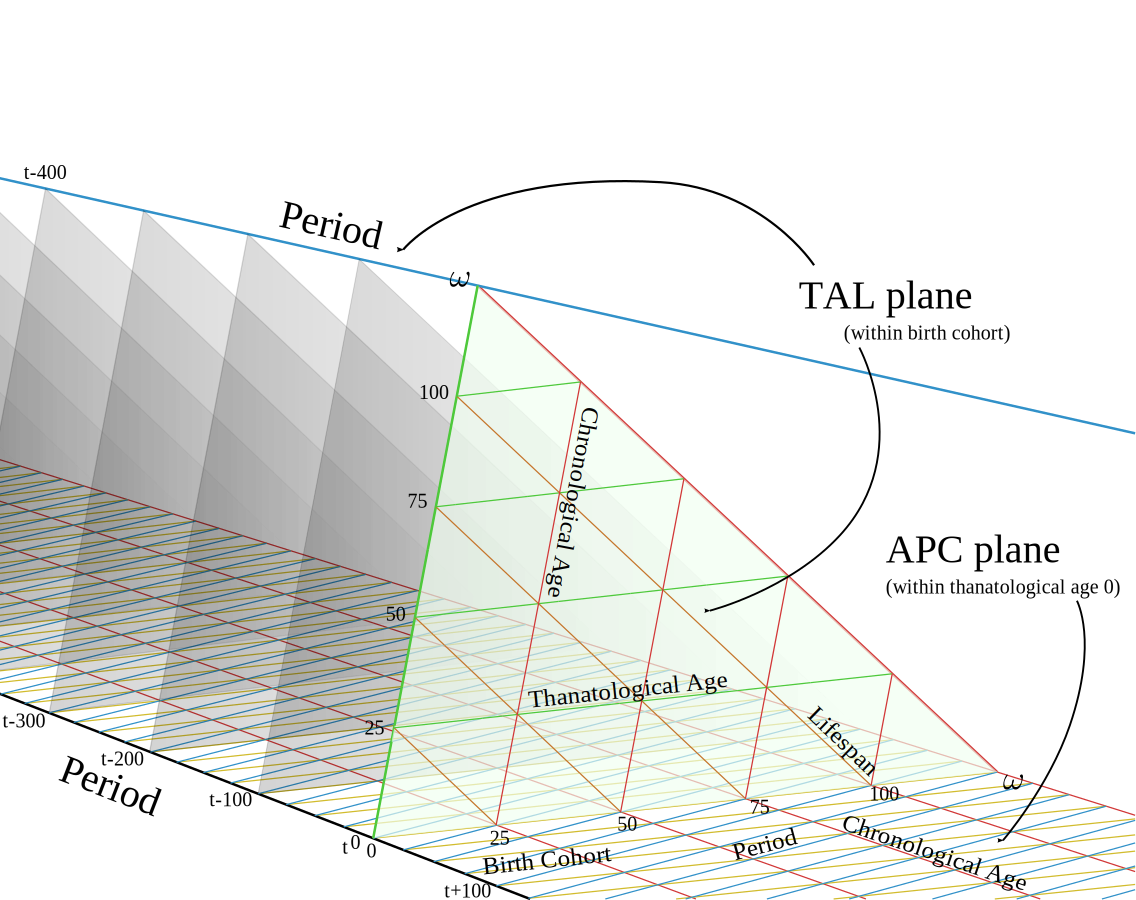
\includegraphics[scale=.5]{Figures/TALisomarkedup2.pdf}
\end{figure}

For example, imagine an infant born in the year 2000. Without further
information, we only know that this infant is located somewhere on the
thanatological age axis of the front TAL plane. If this infant is
destined to die in the year 2100, then the vertical position at birth will be at the axis tick for thanatological age 100. This
person's entire life stays on the 100 lifespan line (labelled),
descending over time towards thanatological age 0. Point A marks the midpoint in
life for this individual, at chronological age 50 (red line, labelled), and
thanatological age 50 (green line). If another APC plane were drawn through thanatological age 50, we would see that point A is in the year 2050. Since all individuals born in the year 2000 complete the same age in the same year, we can
also recuperate the year for point A by following the chronological age 50 line
(red) down to where it meets the blue line for the year 2050. The lifeline
descends downward toward the APC plane for thanatological age 0 at chronological age 100, meeting the year 2100, which determines the
death cohort.

The density and location of imaginary lifelines in this diagram, omitting
migration, is purely a function of birth cohort size and survival. For extinct
cohorts all lifelines can be positioned, but for the 2000 birth cohort this is
not yet the case. Most of the front TAL plane is in the future. One may imagine
yet another plane intersecting this space--- the ``present plane'', which is
identical to the period TAL plane for the present moment. To see how this plane
divides the space, imagine that we are in the year 2025, and follow the blue
line in the APC base inward 25 years to where it meets the red line for chronological age 25, and follow the
red line up the front TAL plane. A single plane cuts through the year
2025 and chronological age 25 from the year 2000 birth cohort. This plane
shifts forward or backward in time to meet the present year. In this particular
plane, the coordinates T, L, and D are uncertain. The period TAL plane $\omega$
years in the past is fully identified, ergo, theoretically the lifespan of each
individual in the time of Lexis is knowable. 

Figure~\ref{fig:apctTAL} could have been drawn with TPD or LCD planes highlighted
as well, but these can still be imagined upon the current rendering. TPD planes
transect this space through any given chronological age, for instance. Imagine a
wall on the left side of the prism, cutting through chronological age 0 (recall
Figure~\ref{fig:TPD}).
In this case, the thanatological age axis is indicated in the very back of the diagram,
calendar time becomes another axis, and death cohort diagonals are not drawn.
TPD planes sequence inward from this first plane, always forming cross-sections
through chronological age. The LCD plane is to be found by rotating the current
prism such that the angle of view is directly down (or up) lifelines, which
would then appear as points (recall Figure~\ref{fig:LCD}).

Further, the two classes of planes drawn
(APC and TAL) could have been drawn and labelled differently.
In practice, the diagram of any triad identity may be drawn held constant for any one of its
three missing indices with no loss of generality. For example, we have
mentioned period (P) and birth cohort (C) TAL planes, but there must also be a
third TAL plane that is held constant for death cohort (D). Another example
of such multiplicity is found in the birth cohort TAL diagram. In this diagram,
lifespan lines can also be interpreted as death cohorts (D), chronological age
lines are also period lines (P), and thanatological age (T) is maintained. This
means that the birth cohort TAL diagram is also a birth cohort TPD diagram.
Multiplicity of this kind can be systematically confirmed, since the C time measure is not part of TPD. To not overly extend this exposition, and to avoid undue confusion, we neither delineate every possible cross-section nor the possible interpretations of each cross-section.
However, in general there are four total ways to cut the
space that are parallel to the faces of the hexad identity, and each cut
has three possible diagram interpretations.

The essential property of this perspective diagram is that lifelines
start and end in parallel, desceding downward and forward in time. A real
population of renewing lives, spread over time and over the typical range of
human lifespans, will tend to fill the entirety of the prism depicted in
Figure~\ref{fig:apctTAL}, and any given point in the prism can be given six
demographic time coordinates, of which two or three are redundant.

\FloatBarrier

\section{Application}
\label{sec:app}
The relationship between the six measures of demographic time is true in the
same sense that mathematics is true: Under linear time it is an internally valid
set of relationships, and this is self-evident. We have mentioned that the
coordinates described here may be useful for the visualization of data, to
enable discovery, and to better inform demographic methods. We have not yet
mentioned how such developments might arise in practice. We therefore give a
schematic overview of our own process of scientific inquiry and reflection that was based this coordinate system, and
that would not have arisen without it. This chain of inquiry is meant to demonstrate the
usefulness of the present framework, but it is far from an exhaustive
application of its potential for other substantive questions, nor is the case
study described in complete rigor. Specifically, we reason that
projections or comparisons of healthy life expectancy (HLE) are in many
cases biased in period prevalence-based models unless one takes into account the
thanatological age pattern of prevalence, as well as mortality differences.

There are three steps in our empirical inquiry. The first step is to visualize
variables on health outcomes using our framework. The second step is to
assess the primary time measures over which health outcomes appear to vary.
Under the assumption that these patterns of temporal variation are empirically regular,
we proceed to develop a method of standardizing health expectancy calculations
for morbidity conditions whose prevalence is more closely related
to thanatological age.
Finally, one can reason that period estimates of health expectancies for certain
health conditions are biased when mortality has been or will-be changing, and
comparisons of HLE between populations with different mortality are also biased.
We conclude that comparisons of health expectancies might be biased in ways not
previously documented.

Let us take the example of self-reported health (SRH). 
 The data come from the RAND version of the US Health and Retirement Study \citep{HRS}. Since this
survey has multiple observations of individuals, as well as a mortality
follow-up, we have each of the six time measures for each observation. Further
methodological details are given by \citet{riffe2015ttd}. 

\begin{figure}[h!] 
\caption{Prevalence of males self-reporting poor health by chronological and
thanatological age, by quinquennial birth cohorts, 1905-1925. (HRS)}
\label{fig:poorsrh}
\centering
\vspace{-1em}
\begin{subfigure}{.46\textwidth}
\centering
\caption{1905}
\vspace{-1em}
\label{fig:srh1905}
\includegraphics[scale=0.32]{Figures/TALapplication/srhpoor1905.pdf}
\end{subfigure}
~
\begin{subfigure}{.46\textwidth}
\centering
\caption{1910}
\vspace{-1em}
\label{fig:srh1910}
\includegraphics[scale=0.32]{Figures/TALapplication/srhpoor1910.pdf}
\end{subfigure}

\begin{subfigure}{.46\textwidth}
\centering
\caption{1915}
\vspace{-1em}
\label{fig:srh1915}
\includegraphics[scale=0.32]{Figures/TALapplication/srhpoor1915.pdf}
\end{subfigure}
~
\begin{subfigure}{.46\textwidth}
\centering
\caption{1920}
\vspace{-1em}
\label{fig:srh1920}
\includegraphics[scale=0.32]{Figures/TALapplication/srhpoor1920.pdf}
\end{subfigure}

\begin{subfigure}{.46\textwidth}
\centering
\caption{1925}
\vspace{-1em}
\label{fig:srh1925}
\includegraphics[scale=0.32]{Figures/TALapplication/srhpoor1925.pdf}
\end{subfigure}
~
\begin{subfigure}{.46\textwidth}
\centering
\caption*{~}
\vspace{-1em}
\label{fig:srhlegend}
\includegraphics[scale=0.32]{Figures/TALapplication/Legend.pdf}
\end{subfigure}
\end{figure} 

Figure~\ref{fig:poorsrh} displays a series of TAL surface plots of SRH
prevalance, each referring to a different quinquennial birth cohort (1905-1909,
etc). The TAL surfaces for
each successive birth cohort are shifted by five years because the observation
window available is from 1992 to 2011 for each cohort. Contour lines in the
surfaces indicate the primary direction of variation. Downward
diagonals indicate lifespans, which the reader may also think of as very
specific birth-death cohorts. These are the diagonals along which lifelines may
be imagined, as suggested in Figures~\ref{fig:TAL} and~\ref{fig:apctTAL}. For each
of these birth-death cohorts we have a prevalence trajectory--- empirical examples of the lifeline morbidity trajectories often conceptually diagrammed in the literature on morbidity compression
\citep[e.g.,][]{fries2005frailty}.
In each surface the primary direction of variation is along thanatological age,
and not chronological age. The prevalence for those with $t$ remaining years of
life is similar in these data, irrespective of chronological age, birth cohort,
or ultimate lifespan.

The marginal chronological age pattern of SRH, as measured
here (the Sullivan curve, \citep{Sullivan1970}), shows an increasing tendency
over age.
However, such an increasing line is a marginal ruse, due to an interaction
between the distribution of lifespans and the relatively fixed underlying
pattern of morbidity seen in Figure~\ref{fig:poorsrh}. These surfaces can indeed
be tidily summarized with a single line, but it is a line over the
thanatological age margin rather than over chronological age. 

Since the patterns for each of these cohorts can be presumed to be the same, any
shifting in the distribution of lifespan ought not produce a change in the
expected years of poor health for a given lifespan. Further, the life years
spent in poor health should also be approximately the same ``on average'', even
if the underlying mortality patterns shift. If morbidity change is a pure
function of thanatological age, an increase in life expectancy should increase
healthy life expectancy by the same amount. This is not the prediction when we
base analyses on the chronological age pattern of self-reported health. An
underlying morbidity pattern this stable would predict improvements in the
marginal chronological age pattern of self-reported health if the lifespan
distribution were to shift to higher ages. This bias in the current status quo
of morbidity measurement and prediction leads to pessimistic morbidity scenarios
when mortality improvements are foreseen, and it undermines health expectancy
comparisons between groups with different mortality \citep{vanRaalte2015HLE}.
Cohort health expectancies are in either case unbiased, but these are also not common.

Using the data from our example surfaces, we can calculate an average prevalence
trajectory with the approach to death and calculate some basic results that
support our case. Let us take the population of US males aged 60 and older, and
assume that the trajectory derived from the Figure~\ref{fig:poorsrh} surfaces
is valid for them.
If we apply this trajectory to the synthetic stationary population of each
year from 1980 and 2010 \citepalias{HMD}, we can calculate the resulting healthy
and unhealthy life expectancies, and compare these with the expectancies that we would have projected assuming the 1980 Sullivan curve.
Total remaining life expectancy at age 60 increased 4.3 years from 17.4 to 21.7
years from 1980 to 2010. Assuming the thanatological trajectory of
morbidity, we calculate healthy life expectancies of 15.7 and 19.9,
respectively, an increase of 4.2 years. Unhealthy life expectancy in this
scenario increased just 0.1 years. Had we used the Sullivan curve from 1980 to
calculate the 2010 values, we would have predicted an increase of 0.7 years in
unhealthy life expectancy, or 39\% versus the 4\% ``observed'' in this
exercise.

This is a large difference in projected morbidity, and it is based on a
relatively minor tweak to standard methodology, itself inspired by viewing data under the conditions
enabled by this temporal framework and adjusting standard demographic methods
to capture the direction of temporal variation in data. There is a wide variety
of prevalence patterns when viewed in this way \citep{riffe2015ttd,
wolf2015disability}, and much empirical and methodological work is still required to verify
that these findings are representative and to understand the consequences for
the standard ways of comparing and projecting HLE. 

Our objective in this application has been
to demonstrate how viewing data under the rigorous conditions enabled by the
time-framework we propose can lead to new scientific understandings of
processes over the life course. Applications for other aspects of the
lifecourse, particular stages of the lifecourse, non-human species on all time
scales, populations of inanimate items on all time scales, and myriad other
substantive areas may gain new insight by applying the relationships contained
in the demographic time identity or its consituent triad identities.

\section{Discussion}

In this paper we describe a relationship between six different measures of
demographic time: chronological age, period, birth cohort, time to death, death
cohort, and individual lifespan. In Section~\ref{sec:dyads2diagrams} we show how
combinations of these time measures imply four triad identities. Each
triad identity consists in simple linear relationship between its three
constituent time measures. We describe how each triad identity can be
extended into a temporal plane, with a characteristic diagram. The four triad
identities underly a family of four diagrams. These diagrams include the
familiar Lexis diagram (Sec~\ref{sec:apc}), but also three either new or
uncommon diagrams.
The TPD diagram (Sec.~\ref{sec:tpd}) relates time of death, period, and time
until death, and is therefore a sort of dual to the Lexis diagram. The TAL
diagram (Sec.~\ref{sec:tal}) relates the three duration measures of time to
death, chronological age, and lifespan, and it may be useful for analyzing patterns that vary over the lifecourse and/or by length of life.
The LCD diagram (Sec.~\ref{sec:lcd}) relates time of birth with time of death
and lifespan, and it may be useful for analyzing patterns that vary over time and by length of life,
but not necessarily over the lifecourse. These four identities and diagrams
relate to one another in a single relationship.

In Section~\ref{sec:gen}
we digress to present a more general event-duration identity framework. These
general terms allow us to present the demographic time hexad identity more
rigorously as a special case of the event-duration framework in
Section~\ref{sec:examples}.
We compare this identity with other relatively complicated temporal
relationships in the literature, including the \citet{lexis1875einleitung}
marriage identity and the illness-death model of \citet{brinks2014lexis}. Some general
properties of temporal identities are mentioned in
Section~\ref{sec:gen} described and elaborated and proven in
Appendix~\ref{app:A}.
In Section~\ref{sec:tetrahedron} we describe how the graph of the demographic time identity is also the graph of a tetrahedron. As a three-dimensional solid, the tetrahedron forms the basis of the three
dimensional extension of the demograhic time identity. Each of the four
faces of the tetrahedron is parallel to one of the four temporal planes.

In Section~\ref{sec:diagram} we render a diagram of the demographic time
identity. We argue that the full three dimensional diagram is not necesarily a
practical way to represent demographic data, but that it forms a useful
reference to understand demographic processes. In general, data structured by
all six demographic time measures can be represented on any of the four diagrams
if controlled properly. In Section~\ref{sec:app} we present a brief
application of this technique to the prevalence of poor self-reported health in
older ages in the United States. Prevalance data are displayed in a series of
TAL surfaces (See Sec.~\ref{sec:tal}) representing the end-of-life experience of
a sequence of five birth cohorts (1905-1925). Together, these surfaces represent
a partial filling of the three-dimensional diagram drawn in
Figure~\ref{fig:apctTAL}. As such, this prevalence data is structured by all six
demographic time measures. To demonstrate the potential utility of this kind of
data structure, we demonstrate (non-rigorously) that the choice of
age-pattern when calculating prevalence-based measures of healthy
life expectancy can have a non-trivial impact on the result.

The contemporary practice of (macro) demography is based on the premise that
vital rates, and other kinds of rates over the lifecourse, are the truest measure of
demographic forces. Rates are paramount because they tend to vary in
empirically regular ways over the life course. The scalings and movements of
primary vital rates fall within a limited range for humans. For this reason, many of the methods of
demography are developed to estimate rates, independent of population composition, or to
partition crude magnitudes into the effects of population age structure and
pure vital rates. Controlling for age like this is in a more general sense
controlling for temporal variation in stocks. To the extent that regular temporal variation
relates to the end of life, or the length of life, common
age-standardization does not fully account for such structure.

An effective way to detect patterns in temporal variation
is via data visualization. The coordinate system proposed in this paper is
conceived as one adequate to capture such variation, and we suggest its use
for visualizing data, probably via small multiples of successive time slices
parallel to any of the four triad identities, similar to that shown in
Figure~\ref{fig:poorsrh}.
Such visualization strategies at this time are exploratory, and this is a
technique that may benefit from further refinement. Further, a cross-section
through the demographic time-space need not be parallel to one of the four
identity-planes.

%In isolation, each of the four triad identities is intuitive. The TPD
%diagram is similar to APC, but it is aligned to time of death rather than time
% of birth. The TAL diagram presents a clear way to classify events over the life course of a cohort. Finally, the LCD diagram can be used to
%structure quantities that vary over time and by length of life.
%Joined together, the relationship between all six time measures is more
%complex than any of the triad identities, but it condenses into a simple
%geometric representation that can be easily derived by ascribing the various
% time measures to the six edges of a tetrahedron. An understanding of how the six time measures relate is key to understanding the temporal structure of demographic processes, which
%itself underlies the comparability of demographic measures.

The techniques used to age-standardize mortality and fertility estimation are at
times applied to other kinds of transitions over the life course. For example,
one may estimate an age pattern to some degenerative disease, or the
ability to carry out some common activities of daily life. However, much of the
regular temporal variation for the prevalence of such conditions is by
time-to-death or lifespan, rather than by chronological age. Apparent chronological age patterns
in such cases are artifactual and do not represent the same kind of
intrinsic meaning as does the \textit{age pattern} of mortality. Further kinds
of temporal standardization must be developed in order to measure and understand
the natural patterns of such conditions over the lifecourse. 
The measurement of
such conditions may benefit from consideration of the framework presented in
this paper. %To this end, Table~\ref{tab:set3} provides all combinations of
%information that are sufficient to derive the full set of six time measures.
Panel surveys with mortality follow-ups already provide the requisite
information, as do linkable registers that include items such as
health measures or proxies and relevant dates of birth, observation, and death.
Other kinds of populations, such as animals or items, may have quite different
data-gathering mechanisms.

%Mortality determines three of the dimensions of
%demographic time, and it therefore makes little sense to model mortality using
%all six time measures. Rather, mortality determines the placement of
%lifelines in the three-dimensional space. Death itself is only representable
%with the endpoints of lifelines, ergo the APC plane through thanatological age
%zero. This full coordinate system instead defines and contains the space
% through which life is lived; any of the six measures may be pertinent in the case of
%conditions and states that vary over and within the lifecourse. An obvious
%application for the present model, given data commonly (and publicly) available
% at this time, are late-life health conditions, although there may be other substantive areas of application.

Furthermore, we believe in the pedagogical value of the framework
introduced in this paper. We hope that the
present inquiry will be useful as a teaching instrument in the same way as APC
diagrams have formed a part of basic demographic education.
The relationship between the six dimensions of demographic time helps situate the APC
paradigm in a broader framework. Just as scientific discovery in general
depends partly on the development of finer optics and instrumentation, we hope
that the framework we describe will prove an instrument to enable new
discoveries in formal, and empirical demography, as well as other diverse fields of
investigation.


% remove appendix, it pushes figures + tables past 10\ldots
%FloatBarrier

%\begin{appendices}
%\section{Variants of tetrahedron graph}
%The graph depicted in Figure~\ref{fig:tet} could be drawn with any of the
%four vertices in the middle of the triangle (as well as other inversions
%and rotations).
%These would all serve equally well to present the same aspects of the model,
% and we have no insight as to whether one of these renditions is more or less
%intuitive. Figure~\ref{fig:app:tet} provides four perspectives on the
%tetrahedron, for the case that this aids in understanding. The reader may make
% a paper tetrahedron, with labeled edges and vertices to be convinced that
%these are identical graphs.
%\begin{figure*}
%        \centering
%        \caption{Some variants of the graph of the APCTDL tetrahedron.} 
%         \label{fig:app:tet}
%        \begin{subfigure}[b]{0.475\textwidth}
%            \centering
%            \includegraphics[width=\textwidth]{Figures/Tetra1.pdf}
%           \caption{\small Vertex \vt{1} in middle. APC Northwest.}
%            \label{fig:tet1}
%        \end{subfigure}
%    \hfill
%        \begin{subfigure}[b]{0.475\textwidth}  
%            \centering 
%            \includegraphics[width=\textwidth]{Figures/Tetra2.pdf}
%           \caption{\small Vertex \vt{2} in middle. APC Northeast.}
%            \label{fig:tet2}
%        \end{subfigure}
%        \vskip\baselineskip
%        \begin{subfigure}[b]{0.475\textwidth}   
%            \centering 
%            \includegraphics[width=\textwidth]{Figures/Tetra3.pdf}
%           \caption{\small Vertex \vt{3} in middle. APC Northwest.}
%            \label{fig:tet3}
%        \end{subfigure}
%        \quad
%        \begin{subfigure}[b]{0.475\textwidth}   
%            \centering 
%            \includegraphics[width=\textwidth]{Figures/Tetra4.pdf}
%            \caption{\small Vertex \vt{4} in middle, as in
%            Figure~\ref{fig:tet}. APC base.}
%            \label{fig:tet4}
%        \end{subfigure}
%    \end{figure*}
%\end{appendices}
%%FloatBarrier
\DeclareRobustCommand{\VAN}[3]{#3}
\bibliographystyle{apacite} % required for demography
%\bibliographystyle{plainnat}
  \bibliography{refs} 
  
\begin{appendices}
\section{Event-duration transformation proofs}
\label{app:A}
This appendix provides some formal support to statements and explanations given
in Section~\ref{sec:gen}. We explain how durations depend on events (and not
vice versa). We list and prove some of the properties of higher-order
identities, such as the number of ways they can be derived, the conditions
for doing so, the number of event and duration measures they contain, and the
number, size, and composition of sub-identities.

\begin{definition} Let $\textbf{p}$ be a vector with $n$ elements where $n \geq
2$ and elements $p_{i=1} \ldots p_n \in \mathbb{R}$. Let $\textbf{d}$ be a vector with $m$ elements such that $\textbf{d}_{ij} = p_i - p_j$ for all $i$ and $j = 1, \ldots, n$ where $i>j$.
\end{definition}

Equivalently $\textbf{d}$ can be expressed as $\text{vech}(\textbf{p}\times
\textbf{1}_n^\textsf{T} - \textbf{1}_n \times \textbf{p}^\textsf{T})$. For ease
of notation we use double indices to index each element of the vector
$\textbf{d}$. The indices $ij$ of the $k^\text{th}$ element of $\textbf{d}$ are
given by $d_{ij} = d_k = p_{i=\left\lfloor \frac
{1}{2}+\sqrt{2k}\right\rfloor+1} - p_{j=k-C\left(\left\lfloor
\frac{1+\sqrt{8k}}{2}\right\rfloor\right)}$ with $C[f(k)]$ being the binomial
coefficient $\binom{f(k)}{2}$.

\begin{theorem} 
The number of elements in $\textbf{d}$ is $m = n(n-1)/2$.
\end{theorem}

\begin{proof} 
Because $d_{ij}$ must satisfy $i > j$ it can be thought of as all
the elements below the subdiagonal of a $n\times n$ matrix of which there are $m = n(n-1)/2$.
\end{proof}

\begin{corollary} 
The sum of the number of elements in $\textbf{p}$ and
$\textbf{d}$ is the number of edges on an $n+1$-polytope, or the number of edges
in a complete graph with $n+1$ vertices.
\end{corollary}

\begin{proof} 
The sum of the number of elements in $p$ and $d$ is $n+m = n + n(n-1)/2$ which
is the number of edges on an $n+1$-polytope.
\end{proof}

Consider the set $P$ of all possible choices of $n$ points in time.

\begin{definition}{$P=\mathbb{R}^n$:}
Let $P=\mathbb{R}^n$ be the standard basis vector-space spanning all
$\textbf{p}$.
\end{definition}

\begin{theorem}
The linear transformation $T_\textbf{A}: P\rightarrow D$ where $D = \mathbb{R}^{n(n-1)/2}$ and $\textbf{A}_T \textbf{p} = \textbf{d}$ is given by

$$
\underbrace{\left[\begin{matrix}
-\textbf{I}_1 & \Big| & \textbf{1}_1 & \Big| & \textbf{0}_{1 \times n-2} \\
-\textbf{I}_2 & \Big| & \textbf{1}_2 & \Big| & \textbf{0}_{2 \times n-3} \\
\vdots & & \vdots & & \vdots \\
-\textbf{I}_{n-1} & \Big| & \textbf{1}_{n-1} & \Big| & \Big(\textbf{0}_{n-1 \times 0}\Big) \\
\end{matrix}\right]}_{\textbf{A}_T}
\times
\underbrace{\left[\begin{matrix}
p_1 \\ \vdots \\ p_n
\end{matrix}\right]}_{\textbf{p}}
=
\underbrace{\left[\begin{matrix}
d_1 \\ \vdots \\ d_{n(n-1)/2}
\end{matrix}\right]}_{\textbf{d}}.
$$

Given \textit{any} $n$ points in time it is always possible to calculate the
durations between any pair of these points. This calculation can be understood
as a linear transformation of the \textit{point-space} $P$ to the
\textit{duration-space} $D$.\footnote{ $\textbf{I}_n$ is the $n \times n$
identity matrix; $\textbf{1}_n$ is a vector with $n$ elements where each element is 1; $\textbf{0}_{m \times n}$ is a $m \times n$ matrix where each element is 0. For notational convenience we allow for a matrix with 0 columns, written $\Big(\textbf{0}_{n \times 0}\Big)$}
\end{theorem}

\begin{proof} $A_T$ is a simple consequence of the definition of
$\textbf{d}$.
\end{proof}

For example, CPD $\textbf{p}$ yields TAL $\textbf{d}$.

\begin{corollary} There exists no linear map $T_\textbf{A}^{-1}: D \rightarrow
P$.
\end{corollary}

Given only a set of $m$ durations it is impossible to identify a single set of
$n$ points in time marking the endpoints of the durations, e.g. given only age one can not derive birth cohort or period.

\begin{proof} $T_\textbf{A}^{-1}$ exists if and only if $\textbf{A}_T^{-1}$ exists. $\textbf{A}_T$ has no inverse since the columns of $\textbf{A}_T$ are always linearly dependent on each other, i.e. the last element in each row of $\textbf{A}_T$ is always the negation of the sum of all the other row elements. Therefore $T_\textbf{A}^{-1}$ does not exist.
\end{proof}

For example, although CPD $\textbf{p}$ yields TAL $\textbf{d}$, TAL does not
yield CPD.

\begin{theorem}
\label{mixing} *(Work in progess)* Something that states that you can transform
 $P^n \leftrightarrow M^n$ where the basis vectors of $M$ are a mixture of point dimensions and duration dimensions.
\end{theorem}
\vt{For example APT yields APCTDL. APT is a mixture of 1 element of
$\textbf{p}$ and 2 elements of $\textbf{d}$. This is different from pure
$P\rightarrow D$}

\vt{TR: I think this theorem can be proved using graph theory as in the
corollary below.}


\begin{definition}{$\textbf{g}$}
Let $\textbf{g} = \left\{p_{i=1,\ldots,n},
d_{k=1,\ldots,m}\right\}$
\end{definition}

\begin{theorem} There are $b = (n+1)^{(n-1)}$ many
ways to choose $n$ elements out of $\textbf{g}$ whoose linear combination yields the
remaining $m$ elements of $\textbf{g}$.
\end{theorem}

\begin{proof}
This is a case of Cayley's formula \citep{cayley1889}, a result from
graph theory which gives the number of possible trees on $k = n+1$ vertices,
$k^{(k-2)}$. In our case, the fully conected graph $\textbf{K}$ with edges
defined by the elements of $\textbf{g}$ according to the third column of
Table~\ref{tab:timelines}, is complete. By Cayley's fomula, the number of
minimal spanning trees on $\textbf{K}$ is equal to $k^{(k-2)}$. Four different proofs of
this result are given in \citet{aigner2010proofs}. The key is to realize that a
minimal spanning tree (MST) on a complete graph will have $k-1$ edges, connected
to each other and all $k$ vertices. As such, the remaining possible edges are
linear combinations of any given MST.
\end{proof}

\begin{corollary}
Each set of $n$ elements from $\textbf{g}$, $\textbf{b}'$ whose linear
transformation yields the remaining $m$ elements of $\textbf{g}$ includes at
least one element of $\textbf{p}$.
\end{corollary}

\begin{proof}
One of the vertices of $\textbf{K}$, say the $k^{\text{th}}$ vertex, is
connected only to edges labelled by the elements of $\textbf{p}$. Since a
spanning tree of $\textbf{K}$ must connect to this vertex to fully connect
$\textbf{K}$, all $b$ valid spanning trees must contain at least one edge
labelled by an element of $\textbf{p}$.
\end{proof}

\vt{TR: is the statement in this proof something that itself also needs to be
proved?-- that one vertex connects only to $\textbf{p}$ If that statement needs
to be proved, is it a lemma? I think this one takes care of the ``mixing''
theorem~\ref{mixing} that is a work in progress above.}

\begin{definition}{$\textbf{G}$}
Let's define $\textbf{G}$ as the identity implied by $\textbf{g}$ whose
graph is $\textbf{K}$.
\end{definition}

\begin{theorem}
An identity $\textbf{G}$ implies a total of $\binom{n+1}{3}$ triad
sub-identities.
\end{theorem}

\begin{proof}
Any set of three vertices from $\textbf{K}$ forms a complete subgraph, and any
complete subgraph implies an identity between its labelled edges. $\textbf{K}$
has $n+1$ vertices, and therefore there are $\binom{n+1}{3}$ ways to select
three vertices from $\textbf{K}$, hence $\textbf{G}$ implies the same number of
triad subidentities.
\end{proof}

\begin{corollary}
Of the $\binom{n+1}{3}$ triad identies implied by $\textbf{G}$, $\binom{n}{2}$
contain exactly two events and one duration.
\end{corollary}

\begin{proof}
This follows by noting that the $n$ event-labelled edges in $\textbf{K}$ connect
to a single vertex. Selecting any two of these $n$ event-labelled edges implies
a tree on three vertices, whose full connection implies a triad identity
composed of the two event edges and one duration edge defined as the time-difference of the
former two. There are $\binom{n}{2}$ ways to select two of of the $n$ event
edges.
\end{proof}

\begin{corollary}
For $n \ge 3$, of the $\binom{n+1}{3}$ triad identies implied by $\textbf{G}$,
$\binom{n+1}{3} - \binom{n}{2} = \binom{n}{3}$ are composed of exactly three
durations.
\end{corollary}

\begin{proof}
This is equivalent to deleting the vertex $k^{\text{th}}$ from $\textbf{K}$, the
vertex that connects only to event-labelled edges, which is constructed
following the middle column of graphs from Table~\ref{tab:timelines} with
vertex labels ignored. This graph has $n$ total vertices, and any set of 3
vertices implies an identity between its three labelled edges, which in this
case by definition can only consist of durations.
\end{proof}

For example, in the demographic time identity there are $n=3$ event measures.
Thus of the $\binom{4}{3} = 4$ triad identities implied $\binom{3}{3} = 1$ of
these identities consist in durations only (TAL). Notice that the measures T and
A change over the lifecourse of an individual, whereas their sum L is fixed.

\begin{definition}{$\textbf{d}_t$} For $\textbf{p}$ that include period
itself, let $\textbf{d}_t$ be the set of duration time measures that change over
the life course and $\textbf{d}_f$ consist in those durations that are fixed attributed of an individual. By
definition, $\textbf{d}_t \cup \textbf{d}_f = \textbf{d}$.
\end{definition}

\vt{awkward: how to say that $\textbf{p}$ includes P? For example, we have P,
but Lexis marriage does not, so this corolarry is only relevant for us and
Brinks here.}

\begin{corollary}
For $n \ge 4$ and For $\textbf{p}$ that include period
itself, of the $d'=\binom{n}{3}$ triad identies whose edges are
labelled only by the elements of $\textbf{d}$, $d^t=\binom{d'}{2}$ of these identities
consist in exactly two elements of $\textbf{d}_t$ and one element of
$\textbf{d}_f$, while $d'-d^t$ of the duration-only triad identities consist in
relationships between three elements of $\textbf{d}_f$.
\end{corollary}

\begin{proof}
$n-2$ of the edges in $K$ are labelled with the elements of $\textbf{d}_t$, and
these all connect to the same vertex. There are therefore $\binom{n-2}{2}$ ways
to form triad identities with them. The third element of each of these
identities cannot connect to the same vertex, and so must be a member of
$\textbf{d}_f$. \vt{(this is almost done, needs a bit more logic)}
\end{proof}



\begin{theorem}
In general, the number of subidentities of size $h$ in $\textbf{G}$ is equal to
$\binom{n+1}{n+1-h} \quad \forall \, h \le n$.
\end{theorem}

\begin{proof}
Vertex deletion on a complete graph results in a complete subgraph. Therefore,
the number of possible complete subgraphs with $h$ vertices is a function of the
number of ways that $n+1-h$ vertices can be deleted from $\textbf{K}$, which is
$\binom{n+1}{n+1-h}$. The labelled edges of each possible complete subgraph
defined in this way represent subidentities.
\end{proof}

For example, from the tetrahedral graph in Figure~\ref{fig:tettet}, we may
delete the vertex that joins the edges labelled A, T, and P, which in effect
deletes these edges, leaving us with the CDL identity. 

\end{appendices}

\end{document}